\subsection{Experimentac\i'on 3: Red de oficina nº 2}
\subsubsection{Descripci\'on del contexto}
Usando nuestro script para analizar la red nos conectamos a una red de oficina mediante Wi-Fi. La misma es de acceso acceso restrigindo y dispone de aproximadamente de 200 terminales conectadas entre computadoras de escritorio y dispositivos m\'oviles. Al ser una oficina cuenta tanto con acces-points para conexiones de wi-fi como bocas para conexi\'on a los switches.

\subsubsection{Descripci\'on de la captura}
La captura se realiz\'o por el lapso de una hora, logrando capturar 196.495 paquetes, de los cuales 7.418 fueron de tipo ARP. Se encontraron paquetes de los siguientes tipos:

\begin{itemize}
\item LLC: 75 \%
\item IP version: 15 \%
\item ARP 3: \%
\item IP version 6: 3 \%
\item 0x5f4, 0x5e0, 0x888e: 4 \% (paquetes desconocidos en total)
\end{itemize}
En este histograma podemos ver la distribuci\'on de los distintos tipos de paquetes observados. \\

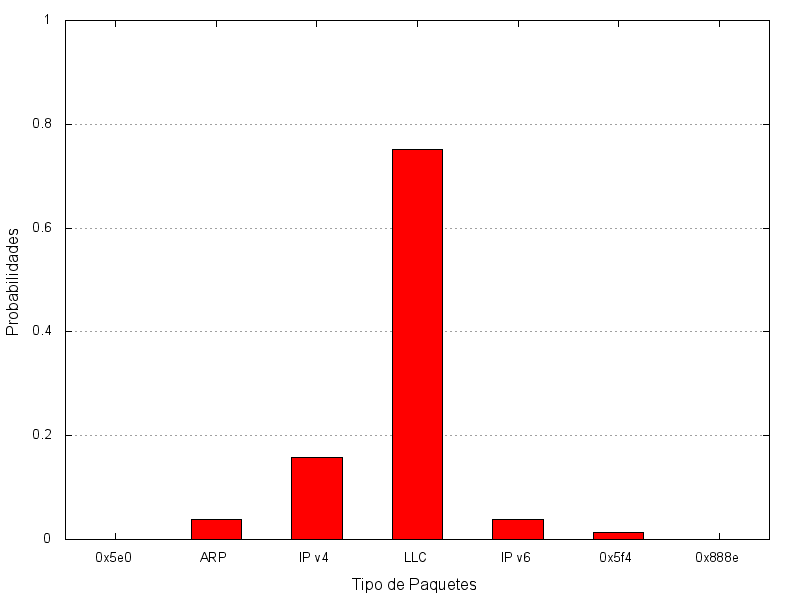
\includegraphics[scale=0.7]{exp3-graficos/s0_oficina_is.png}

En esta muestra caben destacar por un lado la inmensa cantidad de paquetes ''LLC'' en comparaci\'on al resto y los n\'umeros de paquetes desconocidos que en total superan tanto a los paquetes ARP como a los paquetes IP version 6 por separado. \\

Tomando los paquetes ARP vimos m\'as de 90 direcciones IP distintas, lo cual parece un n\'umero particularmente bajo para el tamaño de y carga de trabajo de la red.\\

Aqui vemos un gr\'afico de barras de las IP m\'as significativas de la captura, agrupadas por la presencia que tuvieron.  \\

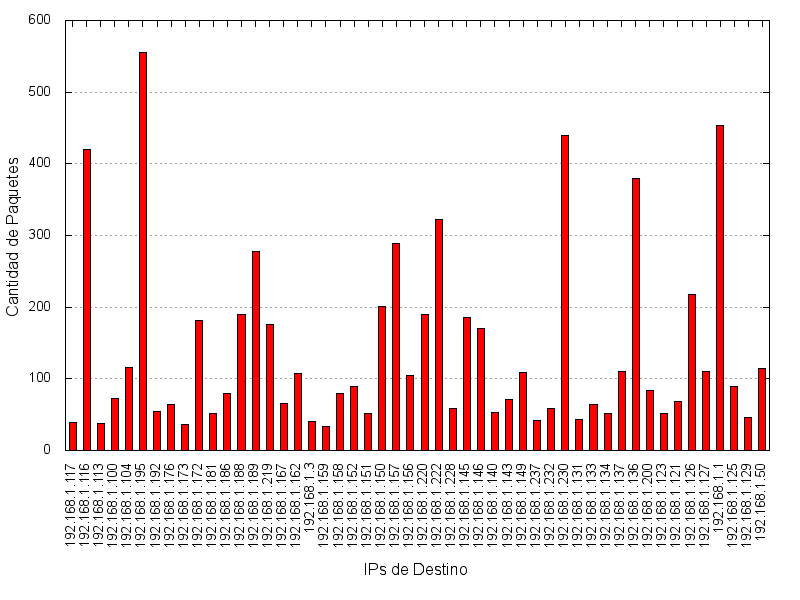
\includegraphics[scale=0.7]{exp3-graficos/s1_oficina_is_pkg.png}

Finalmente las entrop\'ias de nuestras fuentes $S$ y $S_{1}$ fueron 1.1794204458 y 5.47079616204 respectivamente.\\



\subsubsection{An\'alisis de la captura}
El an\'alisis de \'esta de los datos arrojados por la primera fuente generan las siguientes observaciones:

\begin{itemize}
\item LLC es un pr\'otocolo distinguido que supera ampliamente a IPv4/6 y ARP.
\item Tipos de paquetes desconocidos que en total superan a la cantidad de IPV4/6 y ARP por separado.
\end{itemize}

Como vimos en el 1er histograma el 75\% de los paquetes sniffeados desde la terminal conectada por wi-fi son de tipo LLC (Logical Link Control) este paquete es propio del estandard IEEE 802.2 que define el control de enlace l\'ogico para redes de \'area local en el modelo OSI. Este pr\'otocolo se encuentra en la parte superior de la capa de datos y se encarga de manejar los mecanismos de multiplexaci\'on que permite a multiples protocolos coexistir en la misma red. Adem\'as se encarga del control de flujo y de la repetici\'on de requests para manejo de errores. \\\

Actualmente este pr\'otocolo ha ca\'ido en desuso y fue reemplazado por otros como TCP que toman la responsabilidad del flujo y control de errores desde la capa de transporte. Los paquetes LLC contienen en sus headers la informaci\'on de que hacer con un paquete una vez que su frame fue recibido. \\\

Una red con 75\% de participaci\'on de paquetes LLC nos sugiere que la red local es una red de multipunto, que los nodos compiten por el uso de la misma y que se utiliza LLC para que coexistan multiples protocolos de red en un mismo medio (ej: IP, IPX, Decnet and Appletalk). \\\

El segundo punto respecto a la cantidad de paquetes desconocidos puede hacer referencia a paquetes que son recibidos con errores producto del medio de propagaci\'on. \\\


El an\'alisis de los datos arrojados por la segunda fuente nos permiten teorizar sobre los nodos distuinguidos: \\\

Observemos que de un total de m\'as de 7.400 paquetes ARP y m\'as de 90 IP's destino involucradas, el 45\% del destino de esos paquetes fue a parar \'unicamente a un 10\% de las IP's.

\begin{itemize}
\item Probabilidad de 192.168.1.195: 0.0748180102453 - Paquetes: 555
\item Probabilidad de 192.168.1.1: 0.061202480453 - Paquetes: 454
\item Probabilidad de 192.168.1.230: 0.0591803720679 - Paquetes: 439
\item Probabilidad de 192.168.1.116: 0.0566190347803 - Paquetes: 420
\item Probabilidad de 192.168.1.136: 0.0512267457536 - Paquetes: 380
\item Probabilidad de 192.168.1.222: 0.0435427338905 - Paquetes: 323
\item Probabilidad de 192.168.1.157: 0.0389592882178 - Paquetes: 289
\item Probabilidad de 192.168.1.189: 0.0373416015098 - Paquetes: 277
\item Probabilidad de 192.168.1.126: 0.0292531679698 - Paquetes: 217
\end{itemize}

Estos 9 nodos son candidato a nodos distinguidos de la red.
